\documentclass[12pt]{article}

\usepackage{amsmath}
\usepackage{hyperref}
\usepackage{graphicx}
\usepackage{float}
\usepackage{caption}
\usepackage{listings}
\usepackage{xcolor}

% Define a new environment for C++ code
\lstnewenvironment{cpp}
    {\lstset{
        language=C++,
        basicstyle=\small\ttfamily,
        keywordstyle=\color{blue},
        commentstyle=\color{green!40!black},
        stringstyle=\color{orange},
        numbers=left,
        numberstyle=\tiny,
        numbersep=5pt,
        breaklines=true,
        showstringspaces=false,
        backgroundcolor=\color{background},
        frame=tb,
        captionpos=b
    }}
    {}

% Define a new environment for JSON code
\lstdefinelanguage{json}{
    basicstyle=\normalfont\ttfamily,
    numbers=left,
    numberstyle=\scriptsize,
    stepnumber=1,
    numbersep=8pt,
    showstringspaces=false,
    breaklines=true,
    frame=lines,
    backgroundcolor=\color{background},
    stringstyle=\color{stringstyle},
    keywordstyle=\color{keywordstyle},
    commentstyle=\color{commentstyle},
    morestring=[b]",
    morestring=[d]',
    morecomment=[l]{//},
    morecomment=[s]{/*}{*/},
    morekeywords={false,true,null},
    literate=
     *{0}{{{\color{numberstyle}0}}}{1}
      {1}{{{\color{numberstyle}1}}}{1}
      {2}{{{\color{numberstyle}2}}}{1}
      {3}{{{\color{numberstyle}3}}}{1}
      {4}{{{\color{numberstyle}4}}}{1}
      {5}{{{\color{numberstyle}5}}}{1}
      {6}{{{\color{numberstyle}6}}}{1}
      {7}{{{\color{numberstyle}7}}}{1}
      {8}{{{\color{numberstyle}8}}}{1}
      {9}{{{\color{numberstyle}9}}}{1}
}

\definecolor{numberstyle}{rgb}{0.17, 0.57, 0.68}
\definecolor{stringstyle}{rgb}{0.5, 0.3, 0.2}
\definecolor{keywordstyle}{rgb}{0.13, 0.29, 0.53}
\definecolor{commentstyle}{rgb}{0.25, 0.5, 0.37}
\definecolor{background}{rgb}{0.9, 0.9, 0.9}


\setlength{\parskip}{1em}

\begin{document}

\begin{titlepage}
    \centering
    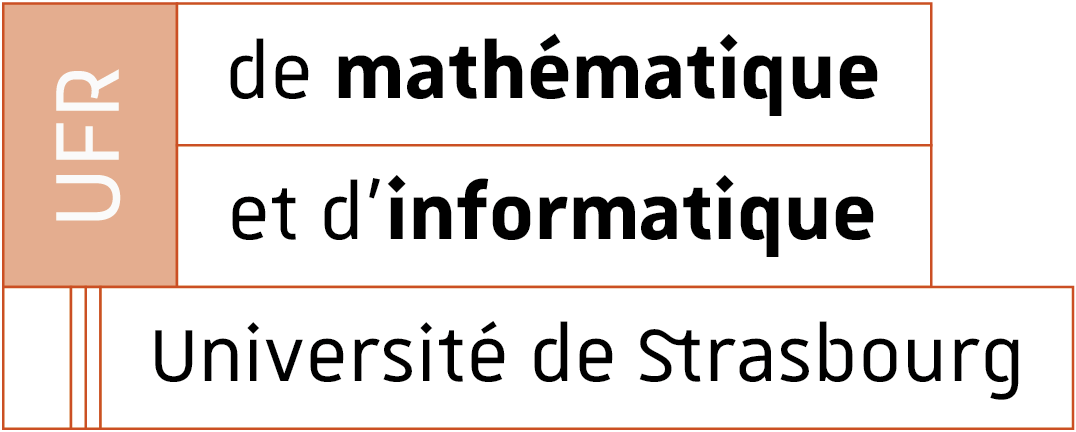
\includegraphics[width=0.5\textwidth]{images/logo_ufr.png}\par\vspace{1cm}
    \vspace{1.5cm}
    {\huge\bfseries ExaMA WP1 - Vegetation\par}
    \vspace{2cm}
    {\Large Giulio Carpi Lapi, Pierre-Antoine Senger\par}
    \vfill
    supervised by\par
    Pierre Alliez and Vincent Chabannes

    \vfill

% Bottom of the page
    {\large Date: \today\par}
\end{titlepage}

\tableofcontents
\newpage

\section{Abstract}
This report explores the integration of vegetation, particularly trees, into 
3D geometric models of urban areas to enhance the accuracy of thermal and 
energy simulations. Leveraging computational modeling advancements, the 
project aims to develop a methodology utilizing tools like GitHub Actions 
for Continuous Integration. The methodology involves retrieving vegetation 
data from OpenStreetMap using the Overpass API and generating 3D models with 
varying levels of detail using CGAL. Feel++, an open-source C++ library, 
will be employed to assess tree shading effects on urban energy simulations. 
Supervised by Pierre Alliez and Vincent Chabannes, the project follows an 
agile methodology with set deadlines. A GitHub repository, 
"2024-m1-vegetation," has been established to facilitate collaboration and 
code review. Roadmaps for project versions ensure timely delivery.

%For the \textbf{V1} version of the report add:

%\begin{itemize}
%   \item Methodology
%   \item Results
%    \item Conclusion
%\end{itemize}

\newpage

\section{Introduction}
Urban areas are complex environments where various factors interact to influence 
microclimates and energy consumption. Among these factors, 
vegetation, particularly trees, plays a crucial role in shaping the urban landscape 
and its environmental characteristics. Trees provide shade, mitigate heat and can
reduce air pollution.

\begin{figure}[H]
    \centering
    \includegraphics[width=0.5\textwidth]{images/TreeShade.png}
    \captionsetup{font={scriptsize}}
    \caption{Urban trees \cite{img:TreeShade}}
\end{figure}

\begin{figure}[H]
    \centering
    \includegraphics[width=0.5\textwidth]{images/heat_street.png}
    \captionsetup{font={scriptsize}}
    \caption{Thermal image of a street in the city. \cite{img:street_thermography}}
\end{figure}

In recent years, advancements in computational modeling have facilitated the 
development of sophisticated tools for simulating the thermal and energy performance 
of urban environments. These tools rely on 3D geometric models that accurately 
represent the built environment, including buildings, roads, and terrain.

\begin{figure}[H]
    \centering
    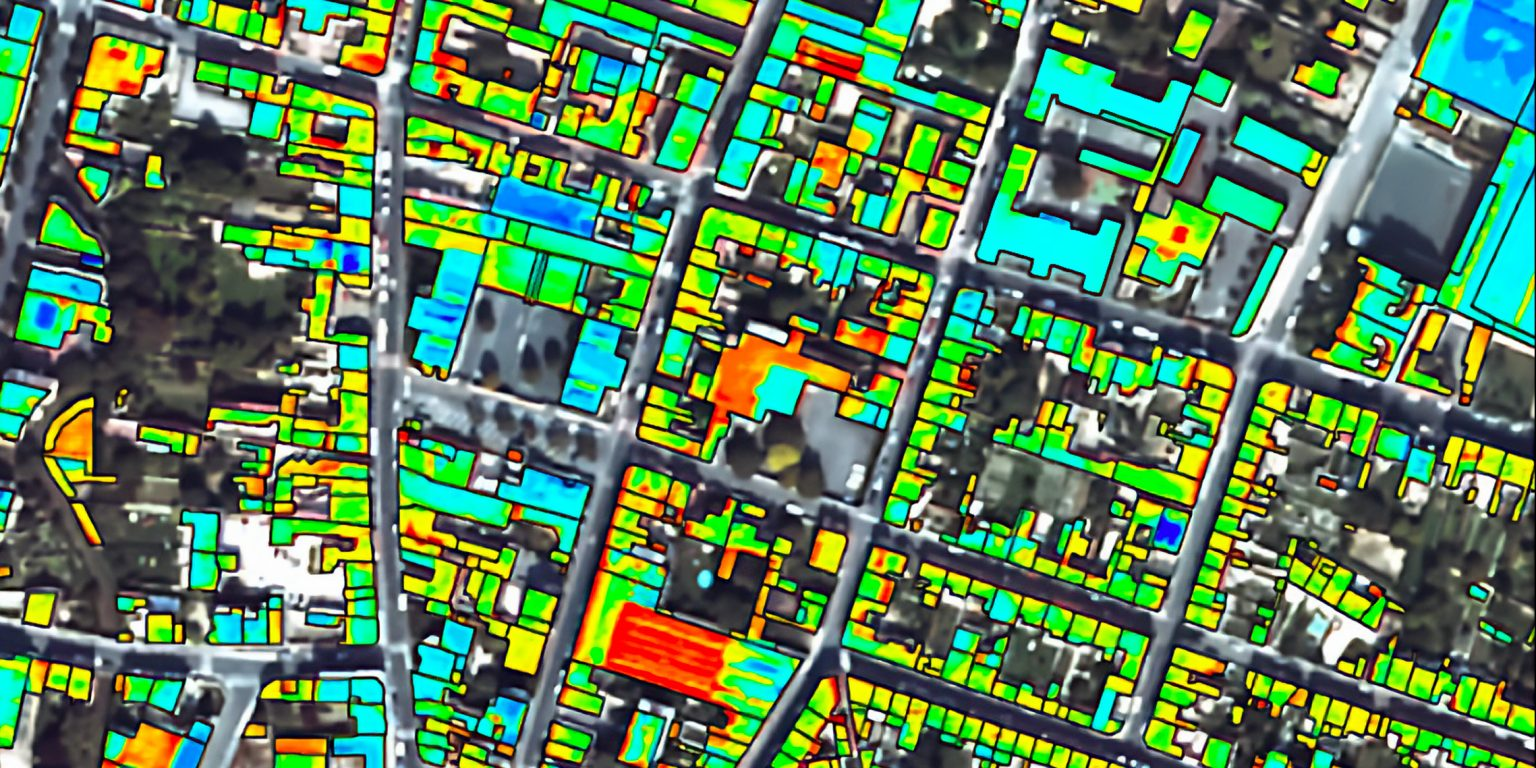
\includegraphics[width=0.5\textwidth]{images/thermographie-aerienne.jpg}
    \captionsetup{font={scriptsize}}
    \caption{Thermal image of a city \cite{img:aerialview}}
\end{figure}

In this context, this project aims to develop a methodology for integrating 
vegetation, particularly trees, into 3D geometric models of urban areas. This
will increase the accuracy of thermal and energy simulations of a neibourhood
or a city.

The vegetation data can be retrieved using the Overpass API for OpenStreetMap.
\vspace{0.5cm}

\begin{figure}[H]
    \centering
    \begin{minipage}{0.45\textwidth}
        \centering
        \includegraphics[width=\textwidth]{images/OSM_logo.png}
        \captionsetup{font={scriptsize}}
        \caption{OpenStreetMap \cite{openstreetmap}}
    \end{minipage}
    \begin{minipage}{0.45\textwidth}
        \centering
        \includegraphics[width=\textwidth]{images/OvAPI_logo.png}
        \captionsetup{font={scriptsize}}
        \caption{Overpass API \cite{overpass}}
    \end{minipage}\hfill
\end{figure}

\newpage
Here is an example of a query that retrieves data for all trees within a 50-meter
radius of the coordinates 48.583194, 7.747951 (Strasbourg city center):

\vspace{0.5cm}
\begin{cpp}
// Set the Overpass API endpoint URL
curl_easy_setopt(curl, CURLOPT_URL, "http://overpass-api.de/api/interpreter");
// Set the Overpass query
std::string query = "[out:json];"
                    "node(around:50,48.583194,7.747951)[\"natural\"=\"tree\"];"
                    "out;";
\end{cpp}
\vspace{0.5cm}

We can then store this data in a .json file. Here's an example
of the outcome for the above query for just one tree:

\vspace{0.5cm}
\begin{lstlisting}[language=json]
{
  "version": 0.6,
  "generator": "Overpass API 0.7.62.1 084b4234",
  "osm3s": {
    "timestamp_osm_base": "2024-03-27T13:32:34Z",
    "copyright": "The data included in this document is from www.openstreetmap.org. The data is made available under ODbL."
  },
  "elements": [
{
  "type": "node",
  "id": 10162019518,
  "lat": 48.5831903,
  "lon": 7.7477189,
  "tags": {
    "circumference": "172.788",
    "diameter_crown": "20",
    "genus": "Platanus",
    "height": "18",
    "natural": "tree",
    "ref": "16279",
    "source": "data.strasbourg.eu - patrimoine_arbore",
    "source:date": "2022-01-02",
    "species": "Platanus acerifolia x"
  }
}

  ]
}
\end{lstlisting}
\vspace{0.5cm}

From the .json file we can then generate à C++ class called
Tree for a better management of all the recovered data.
From this library, we will be able to generate 3D models (meshing)
of different levels of detail (LOD) thanks to the CGAL library.


CGAL is an open source software project that provides easy access to efficient
and reliable geometric algorithms in the form of a C++ library which is used
in various areas needing geometric computation.\cite{cgal}

\begin{figure}[H]
    \vspace{1.5cm}
    \centering
    \includegraphics[width=0.5\textwidth]{images/cgal_logo.png}
\end{figure}

Softwares like MeshLab, an open source system for processing and editing 3D
triangular meshes\cite{meshlab}, will allow us to visualize the 3D models
generated with the help of CGAL.

Starting with LOD0, which represents the least detailed version of the model,
we will progressively complexify it to LOD1 and LOD2.
Each level adds a layer of complexity, making it more resource-intensive to render.

Here's an example of different LODs for a tree model created
with CGAL:

\begin{figure}[H]
    \centering
    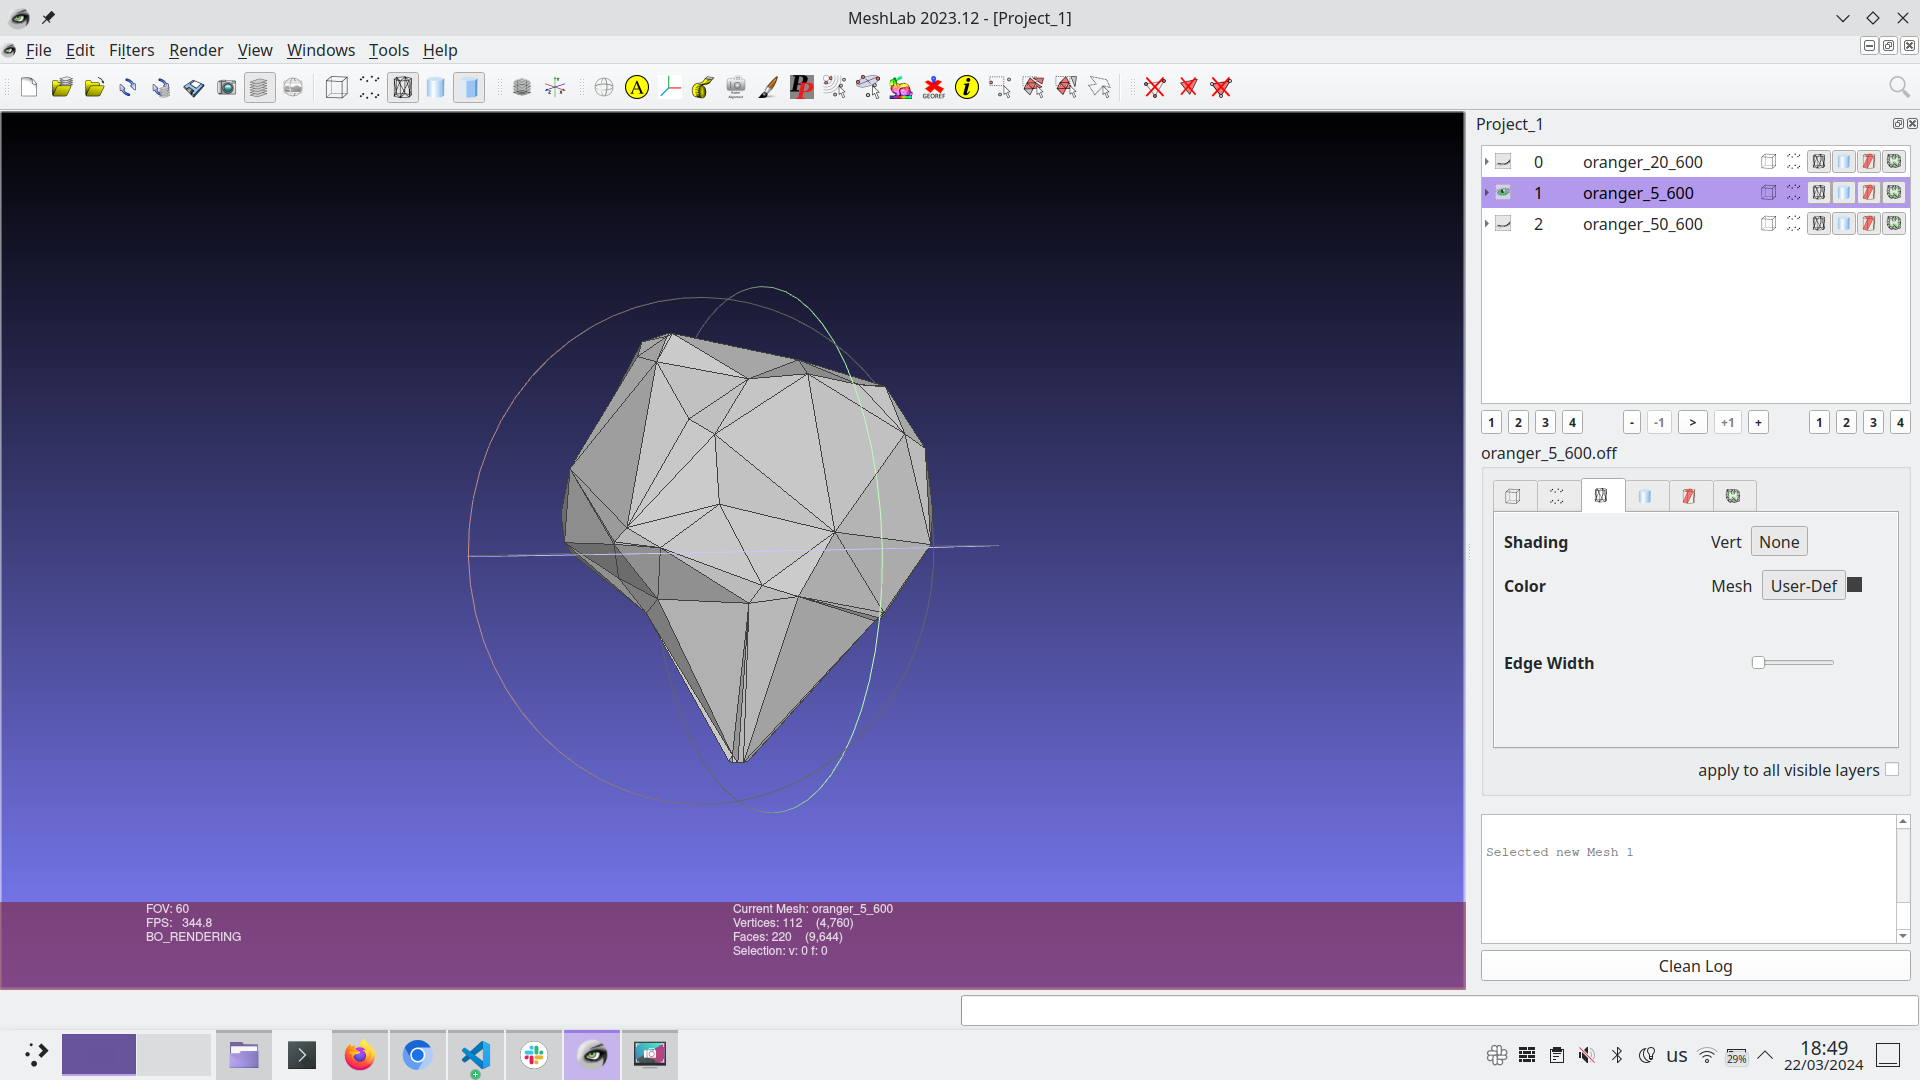
\includegraphics[width=0.5\textwidth]{images/LOD0.png}
    \captionsetup{font={scriptsize}}
    \caption{LOD0}
\end{figure}

\begin{figure}[H]
    \centering
    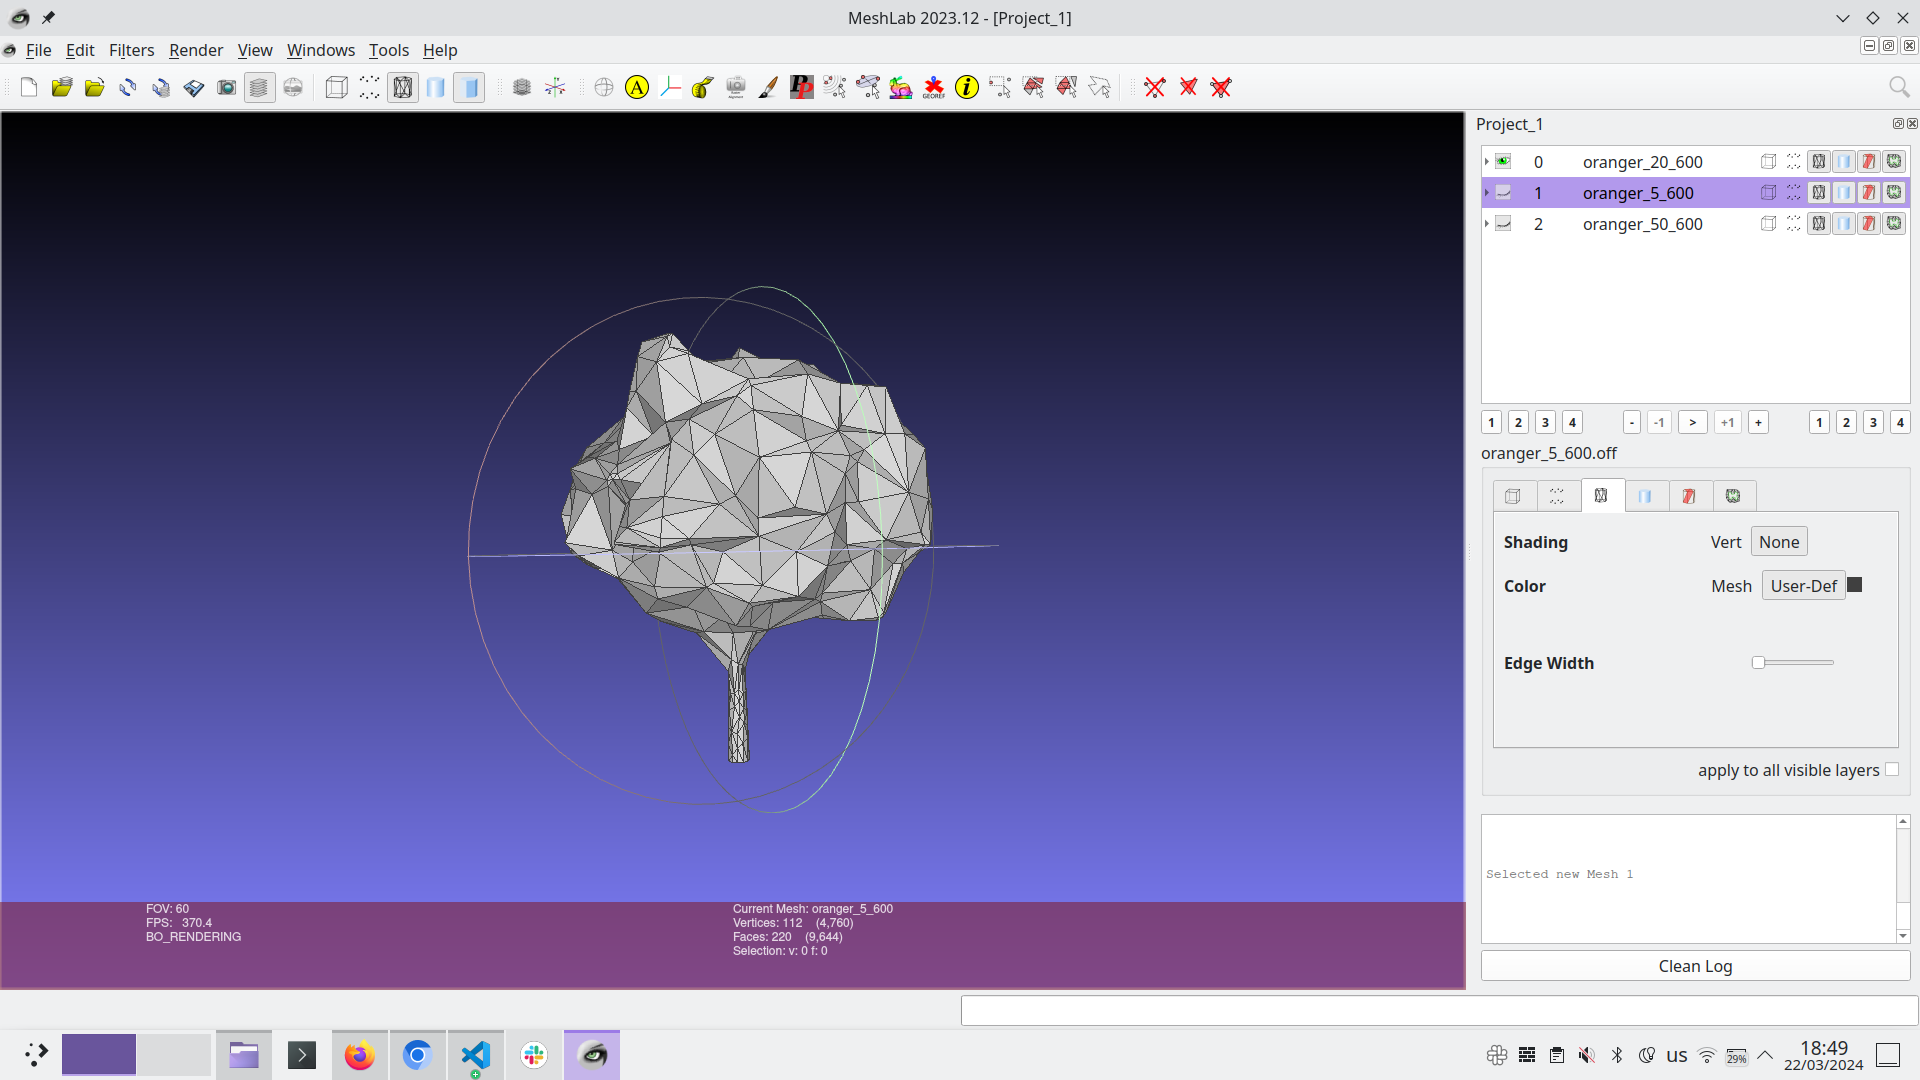
\includegraphics[width=0.5\textwidth]{images/LOD1.png}
    \captionsetup{font={scriptsize}}
    \caption{LOD1}
\end{figure}

\begin{figure}[H]
    \centering
    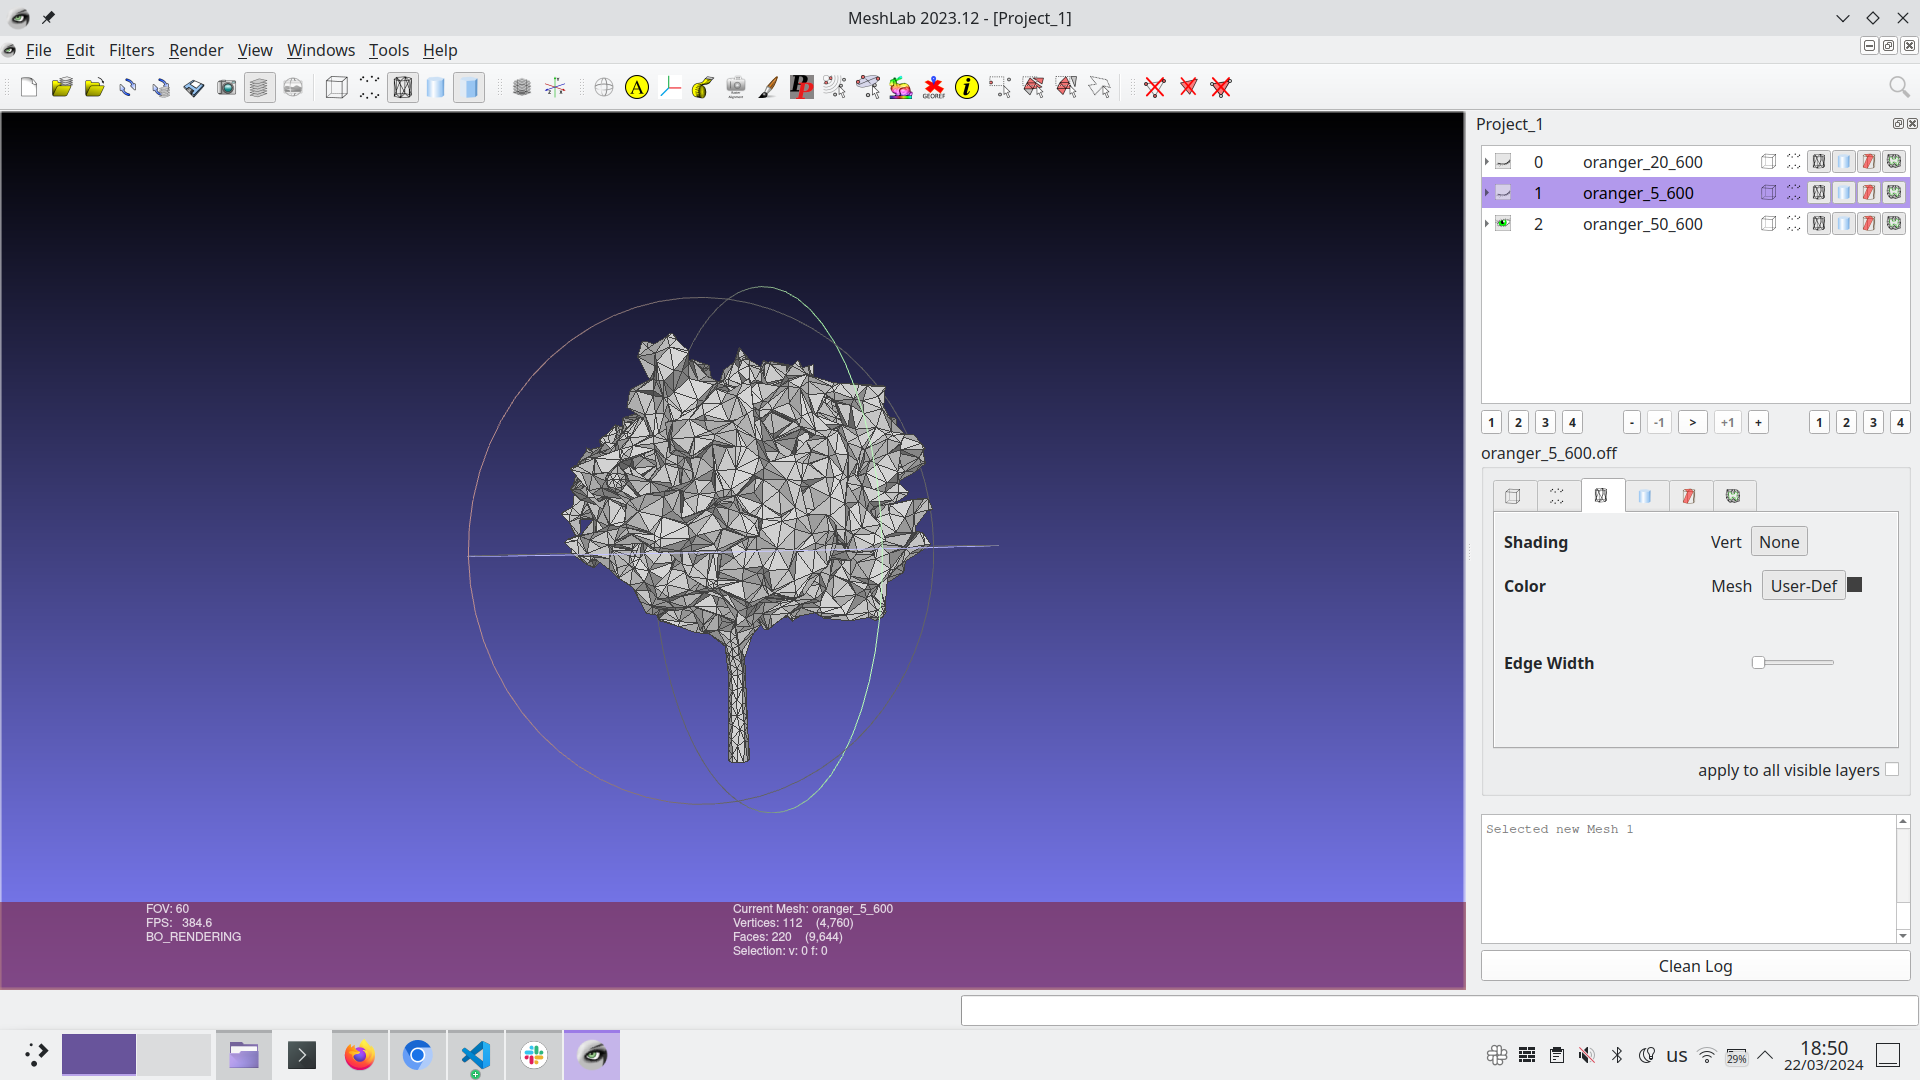
\includegraphics[width=0.5\textwidth]{images/LOD2.png}
    \captionsetup{font={scriptsize}}
    \caption{LOD2}
\end{figure}

\newpage
We will utilize Feel++, an open-source C++ library, to assess how tree shading
impacts urban energy simulations. This library is well-suited for solving
Partial Differential Equations (PDEs), which are crucial for calculating
light and shade effects on 3D objects\cite{feel++}.

The project is supervised by Pierre Alliez Senior Researcher at Inria center
at Côte d'Azur University and by Vincent Chabannes research engeneer at the
University of Strasbourg. We will have weekly meetings with them to discuss
the progress of the project. The deadlines we have set are the following:

\begin{itemize}
    \item \textbf{V0} : due by March 26, 2024
    \item \textbf{V1} : due by April 23, 2024
    \item \textbf{V2 - Final} : due by May 28, 2024
\end{itemize}

We've established a GitHub repository named "\textbf{2024-m1-vegetation}" on the 
Master page to facilitate collaboration, issue tracking, and ongoing code 
review. Additionally, we'll leverage tools like GitHub Actions for Continuous 
Integration (CI) to ensure comprehensive testing and efficient deployment of 
changes.

Adopting the agile methodology for this project, we've outlined the 
following roadmap:


\begin{figure}[H]
    \centering
    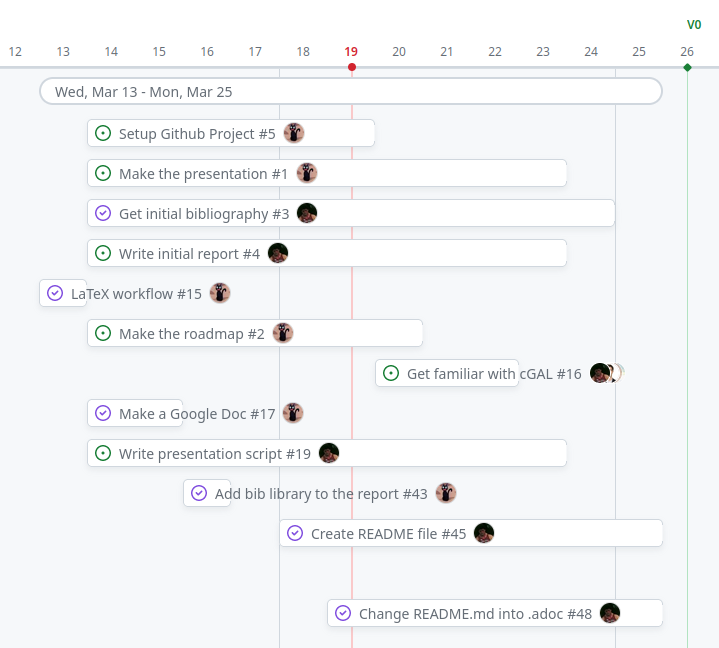
\includegraphics[width=0.5\textwidth]{images/roadmap_v0.png}
    \captionsetup{font={scriptsize}}
    \caption{Roadmap v0}
\end{figure}

\begin{figure}[H]
    \centering
    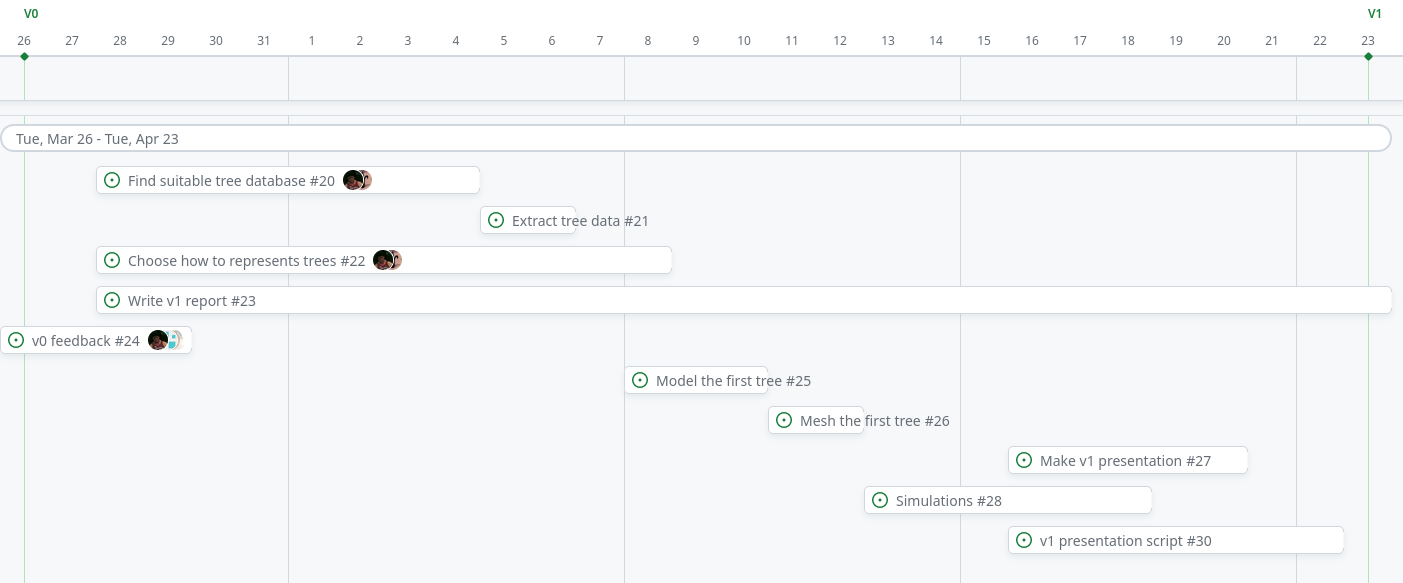
\includegraphics[width=0.5\textwidth]{images/roadmap_v1.png}
    \captionsetup{font={scriptsize}}
    \caption{Roadmap v1}
\end{figure}

\begin{figure}[H]
    \centering
    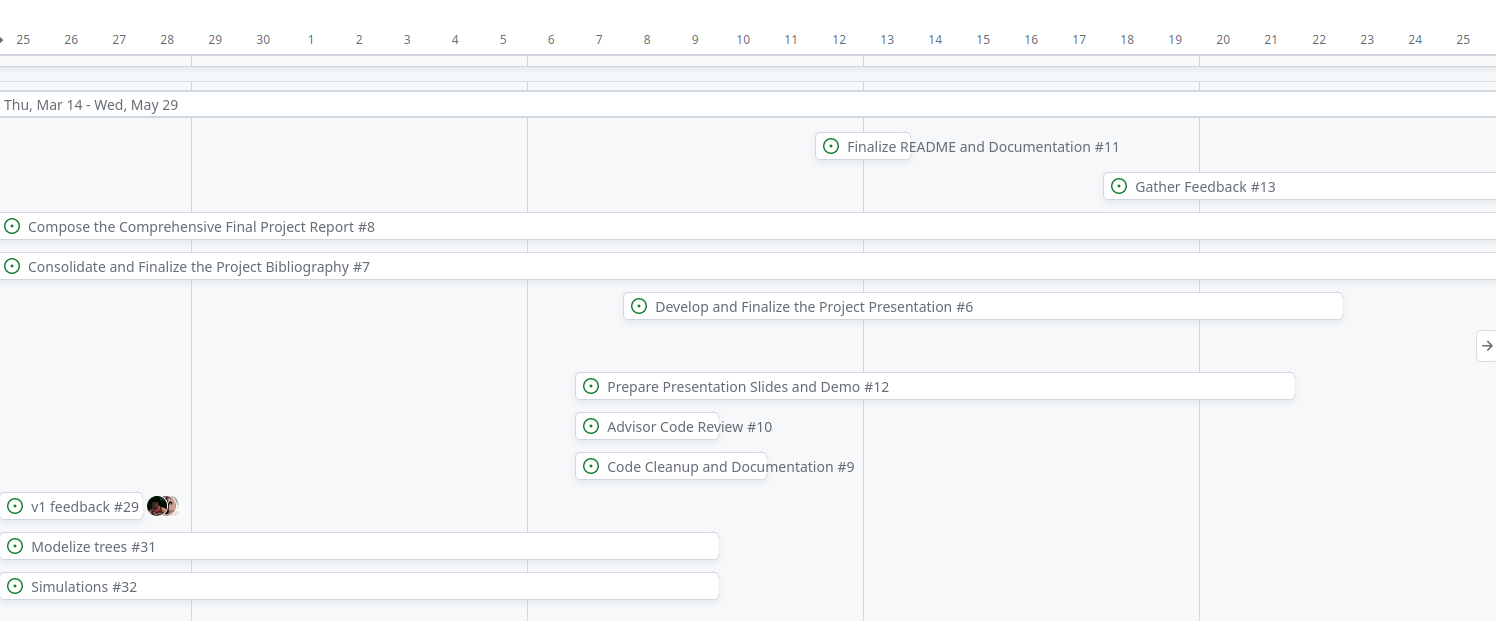
\includegraphics[width=0.5\textwidth]{images/roadmap_v2.png}
    \captionsetup{font={scriptsize}}
    \caption{Roadmap v2}
\end{figure}

This will help us to keep track of the progress of the project and to make sure
we are going to deliever the respective versions on time.

This project will be developed in C++.

\newpage
\section{Literature Review}

\newpage

\section{Methodology}

\newpage

\section{Results}

\newpage

\section{Conclusion}

\newpage

\section{References}
\bibliographystyle{plain}
\bibliography{references}

\end{document}